% intro
\section{Part 2: Crowd-Sourcing for Question Generation}
\label{sec:crowdqa}

Some tasks cannot be automatically generated from templates and require human discretion.  
%
One cost-efficient, scalable pool for human input are crowd-sourcing platforms, specifically Mechanical Turk~\citep{buhrmester2016amazon}.
%
We summarize a data collection project that used unspecialized workers to rewrite trivia questions.  

%Question Answering (\abr{qa}) is an \textsc{ai} complete
%problem~\citep{webber-92}, but existing \abr{qa} datasets do not rise
%to the challenge: they lack key \textsc{nlp} problems like anaphora
%resolution, coreference disambiguation, and ellipsis resolution.
%
%The logic needed to answer these types of questions requires deeper
%\textsc{nlp} understanding that simulates the context in which humans
%naturally answer questions.


\begin{figure}[t!]
	\centering
	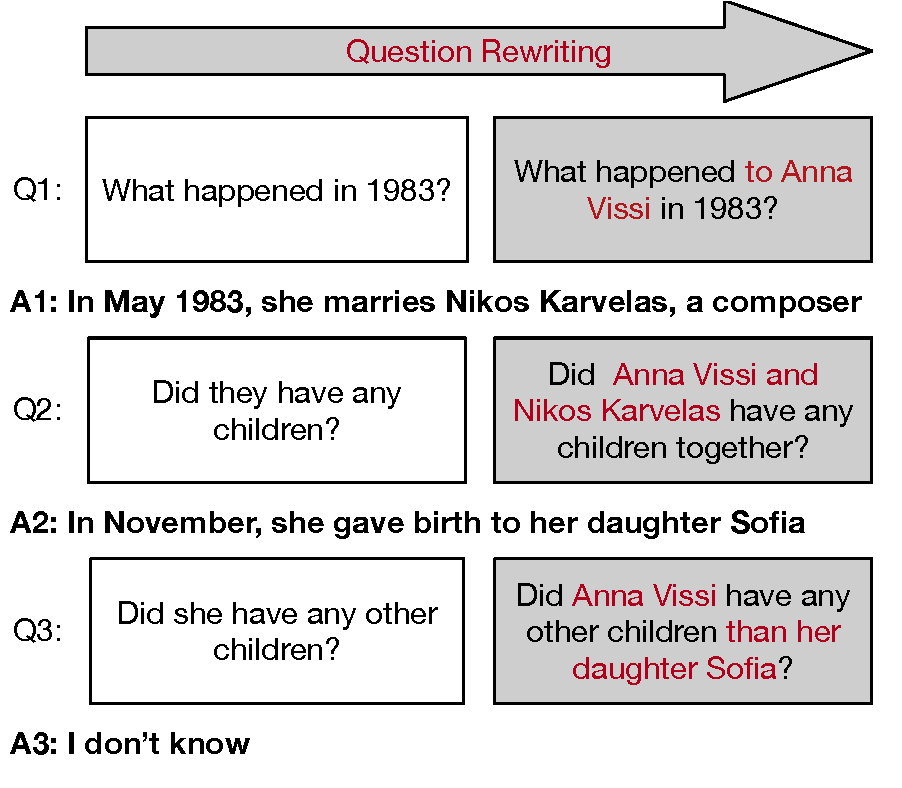
\includegraphics[width=.8\linewidth]{denis_proposal/figures/F1_OmniVersion.pdf}
	\caption{Question-in-context rewriting task. The input to each step
	is a question to rewrite given the dialog history which consists
	of the dialog utterances (questions and answers)  
	produced before the given question is asked. The output is an equivalent, context-independent paraphrase of the input question.}
	\label{fig:example_convo}
\end{figure}

Background Section~\ref{sec:qa} distinguishes between machine reading comprehension (\abr{mrc}) and the nascent area of conversational question answering (\abr{cqa}).  
%
However, we observe that \abr{cqa} questions can be rewritten as stand-alone \abr{mrc} questions and provide additional training data.  
%
We reduce challenging, interconnected \abr{cqa} examples to
independent, stand-alone \abr{mrc} to create
\name{}---\textbf{C}ontext \textbf{A}bstraction: \textbf{N}ecessary
\textbf{A}dditional \textbf{R}ewritten \textbf{D}iscourse---a new
dataset\footnote{\url{http://canard.qanta.org}} that rewrites
\abr{\quac}~\citep{choi2018quac} questions.
%
We crowd-source context-independent paraphrases of \abr{\quac}
questions and use the paraphrases to train and evaluate
question-in-context rewriting.
%
In the process, we observe the behavior of crowd users and the quality of their output.  
 %to simulate the interactive learning setup.

%\jbgcomment{``interactive learning setup'' doesn't make much sense to me}

%%%
%
%Other than being a pre-processing step for sequential
%question answering, the question-in-context paraphrasing task
%can be used for evaluating general models for dialogue understanding and
%sequence models for capturing long-term dependencies.
%As explained in Section~\ref{sec:data}, we made sure the reference
%paraphrases in our dataset are mostly copied spans from the
%conversation history, which makes BLEU~\citep{papineni2002bleu}
%a reliable measure for evaluating how different paraphrasing models
%perform on the task.

%%%%

Section~\ref{sec:data} constructs \name{}, a new dataset of
question-in-context with corresponding context-independent
paraphrases.
%
Section~\ref{sec:analysis} analyzes our rewrites (and the underlying
methodology) to understand the linguistic phenomena that make
\abr{cqa} and using crowd-sourcing for \textit{generation} difficult.


%%DENISTODO
%DONE\jbgcomment{The last sentence in above paragraph is devoid of content;
 % either cut or flesh out so that it wouldn't fit in any paper.}
